\documentclass[12pt, a4paper]{article}
\usepackage[utf8]{inputenc}
\usepackage[T1]{fontenc}
\usepackage[french]{babel}
\usepackage{geometry}
\usepackage{graphicx}
\usepackage{amsmath}
\usepackage{amssymb}
\usepackage{booktabs}
\usepackage{array}
\usepackage{enumitem}
\usepackage{xcolor}
\usepackage{ulem}
\usepackage{float}
\usepackage{caption}
\usepackage{adjustbox}
\usepackage{tikz}
\usepackage{enumitem}
\usepackage{fancyhdr} % Ajout du package pour les en-têtes

\usetikzlibrary{calc, shapes.geometric}
\geometry{margin=2cm}

% Configuration de l'en-tête
\pagestyle{fancy}
\fancyhf{} % Efface les en-têtes et pieds de page par défaut
\renewcommand{\headrulewidth}{0.4pt}
\renewcommand{\headrule}{\hrule width\headwidth height\headrulewidth}
\fancyhead[C]{\rule{\textwidth}{0.4pt}} % Ligne centrée
\fancyhead[R]{\textit{Investigation numérique}} % Texte à droite
\fancyfoot[C]{\thepage} % Numéro de page centré

% Marges réduites

\definecolor{blue1}{RGB}{0, 51, 102}
\definecolor{blue2}{RGB}{0, 102, 204}
\definecolor{gray1}{RGB}{240, 240, 240}

\geometry{margin=2.5cm}

\begin{document}
	\begin{titlepage}
	
	% Bordure autour de la page
	\begin{tikzpicture}[remember picture, overlay]
		\draw[line width=2pt, black] 
		($(current page.north west) + (0.5cm,-0.5cm)$) rectangle 
		($(current page.south east) + (-0.5cm,0.5cm)$);
	\end{tikzpicture}
	
	\centering
	
	% SOLUTION FONCTIONNELLE : Tableau avec alignement en bas
	\begin{tabular}{@{}p{0.25\textwidth}@{\hspace{2cm}}c@{\hspace{0.5cm}}p{0.5\textwidth}@{}}
		% Colonne de gauche (Français) - ALIGNÉ EN BAS
		\begin{minipage}[t][5cm][b]{0.39\textwidth}
			\raggedright
			\begin{center}
				{\small \textbf{RÉPUBLIQUE DU CAMEROUN}}\\
				{\small \textbf{******}}\\
				{\small \textbf{UNIVERSITÉ DE YAOUNDÉ}}\\
				{\small \textbf{I}}\\
				{\small \textbf{******}}\\
				{\small \textbf{ÉCOLE NATIONALE SUPÉRIEURE POLYTECHNIQUE}}\\
				{\small \textbf{******}}\\
				{\small \textbf{DÉPARTEMENT DU GÉNIE INFORMATIQUE}}\\
			\end{center}
		\end{minipage}
		&
		% Colonne du centre (LOGO EN BAS)
		\begin{minipage}[t][5cm][b]{0.2\textwidth}
			\centering
			
			\vspace*{\fill} % Pousse le logo vers le bas
			
\includegraphics[width=\textwidth, height=3cm]{logo.jpeg}
			\vspace*{\fill} % Espace en bas
		\end{minipage}
		&
		% Colonne de droite (Anglais) - ALIGNÉ EN BAS
		\begin{minipage}[t][5cm][b]{0.36\textwidth}
			\raggedright
			\begin{center}
				{\small \textbf{REPUBLIC OF CAMEROON}}\\
				{\small \textbf{******}}\\
				{\small \textbf{UNIVERSITY OF YAOUNDE I}}\\
				{\small \textbf{******}}\\
				{\small \textbf{NATIONAL ADVANCED SCHOOL OF}}\\
				{\small \textbf{ENGINEERING}}\\
				{\small \textbf{******}}\\
				{\small \textbf{DEPARTMENT OF COMPUTER ENGINEERING}}\\
			\end{center}
		\end{minipage}
	\end{tabular}
	
	\vspace{1.5cm}
	
	% Ligne séparatrice
	\noindent\rule{0.9\textwidth}{0.8pt}\\
	\vspace{0.5cm}
	
	% Thème
	\vspace{0.8cm}
	{\Large \textbf{RESUME DU COURS}}\\
	\vspace{0.5cm}
	{\Large \textbf{"THEORIES ET PRATIQUES DE L'INVESTIGATIONS NUMERIQUES"}}\\
	\vspace{0.8cm}
	
	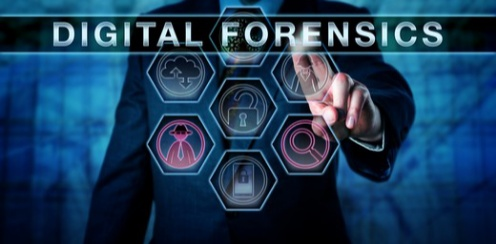
\includegraphics[width=0.5\textwidth]{For.jpeg}
	% Ligne séparatrice
	\noindent\rule{0.9\textwidth}{0.8pt}\\
	\vspace{1.5cm}
	
	% Informations étudiant
	\begin{tabular}{@{}>{\bfseries}l l@{}}
		\vspace{0.5cm}
		Réalisé par : & \textbf{NANTIA ZAGUE AXEL FRISKYL} \\
		\vspace{0.5cm}
		Matricule : & \textbf{22P105} \\
		\vspace{0.5cm}
		Spécialité : & \textbf{Cybersécurité et Investigation Numérique (CIN)} \\
		\vspace{0.5cm}
		UE : & \textbf{Introduction aux techniques de l'Investigations Numériques} \\
		\vspace{0.5cm}
		Sous la supervision de : & \textbf{Mr. MINKA MI NGUIDJOI Thierry Emmanuel} \\
		\vspace{0.5cm}
		Année académique : & \textbf{2025/2026} \\
	\end{tabular}
	
\end{titlepage}

% Page de garde sans en-tête
\thispagestyle{empty}
\newpage


\title{\textbf{Reponses aux questions du chapitre I}}
\author{}
\date{}


	
	\maketitle
	
	\section*{Partie 1 : Fondements Philosophiques et Épistémologiques}
	
	\subsection*{I. Analyse Critique du Paradoxe de la Transparence}
	
	\subsubsection*{Question 1 : Dissertation de 500 mots sur le paradoxe identifié par Byung-Chul Han}
	
	Byung-Chul Han dépeint dans ses travaux un paradoxe majeur caractérisant les sociétés contemporaines, que l'on peut qualifier de « paradoxe de la transparence ». Selon lui, la montée en puissance de la transparence numérique, sociale et médiatique ne libère pas l'individu mais l'enferme paradoxalement dans une forme nouvelle de contrôle et d'aliénation. Ce paradoxe se manifeste dans une société où tout est appelé à être visible, exposé, accessible, au nom d'une liberté affichée, mais où cette transparence obligée viole la vie privée, nivelle les différences et érode la confiance.
	
	Au cœur du paradoxe se trouve l'ambiguïté de la transparence : elle promet l'émancipation par la connaissance et la visibilité, mais réalise souvent une uniformisation et une instrumentalisation des individus. Dans la société qu'il nomme « société de transparence », l'individu est sommé de se dévoiler, de rendre compte de chaque aspect de sa vie, de ses opinions, de ses moindres actions. Cette injonction provoque une « tyrannie de la visibilité » où chacun devient à la fois acteur et spectateur d'un panoptique global digital. Byung-Chul Han souligne que la transparence contemporaine n'est pas une expression de la négativité, c'est-à-dire de la différence, du secret ou du refus. Au contraire, elle est une société positive qui lisse, homogénéise, nivelle les singularités. Cette positivité exaltée, liée à l'hypercapitalisme numérique, ne produit pas de communautés vivantes capables d'actions communes, mais seulement des regroupements d'individus isolés ayant en commun leur exposition et leur consommation d'attention. La notion même de vérité s'en trouve modifiée, éclatée en une multiplication de sources et de récits concurrentiels, ce qui brouille la distinction entre vrai et faux. Ce paradoxe porte aussi sur la liberté. Alors que les anciens systèmes de contrôle reposaient sur la surveillance négative et la restriction, la société de transparence promet la liberté absolue, fondée sur la visibilité totale. Mais cette liberté apparente est en fait une forme nouvelle de domination, un contrôle par la transparence généralisée où la liberté devient synonyme d'auto-exposition et d'auto-exploitation. Byung-Chul Han formule ainsi une dialectique de la liberté où la liberté apparaît sous la forme du contrôle.
	
	Les conséquences sociales et psychiques de ce paradoxe sont notables : épuisement, anxiété, solitude dans l'hyper exposition, fuite dans le repli identitaire et la bulle de filtre où l'on ne rencontre plus que soi-même et ses semblables. La société de transparence conduit à une négation de l'altérité et de la différence, base pourtant nécessaire à une véritable vie sociale et politique.
	
	Pour dépasser ce paradoxe, Byung-Chul Han invite à une réintroduction de la négativité, du secret et de l'intimité comme conditions de la liberté réelle. Il plaide pour une société capable d'équilibrer transparence et opacité, visibilité et confidentialité, afin de préserver la singularité et la liberté humaine. Ce mouvement implique aussi une critique de l'hyper capitalisme numérique et de ses effets déshumanisants.
	
	En conclusion, le paradoxe de la transparence décrit par Byung-Chul Han révèle le double visage de la société numérique : une promesse de liberté par la visibilité qui se transforme souvent en aliénation sous contrôle. Cet impensé de l'émancipation numérique appelle à repenser les conditions de la transparence, pour que celle-ci ne devienne pas une nouvelle forme d'oppression mais un véritable levier de liberté humaine et collective. La conscientisation de ce paradoxe ouvre la voie à une critique éthique nécessaire face aux défis contemporains du numérique.
	
	\subsubsection*{Question 2 : Appliquez ce paradoxe à un cas concret d'investigation}
	
	Imaginons une enquête policière sur un vol commis dans une entreprise. Les enquêteurs numériques demandent à accéder aux enregistrements vidéo des caméras de surveillance ainsi qu'aux historiques de connexion informatique des employés pour identifier le coupable. La transparence veut ici que toutes les données utiles soient accessibles pour révéler la vérité. Cependant, certaines vidéos captent également des moments privés d'employés non liés au vol comme des une vidéo d'un personnel entrain de visionner les « Gesiers » dans son PC, et les historiques de connexion contiennent des informations personnelles sensibles (mails privés, sites visités). La divulgation intégrale de ces données porterait atteinte au droit à la vie privée des personnes. Ici, le paradoxe se manifeste : pour révéler la vérité sur le vol, il faut une transparence des preuves, mais cette transparence risque de violer la vie privée d'innocents. L'investigateur numérique doit donc filtrer, anonymiser ou protéger les parties non pertinentes des données afin de respecter l'intimité, tout en permettant l'accès aux informations importantes. Par exemple, les vidéos peuvent être visionnées en privé par les enquêteurs sans publication publique, et les historiques nettoyés des données personnelles. Cette stratégie respecte le paradoxe du paradoxe : équilibre entre la quête de vérité transparente et la protection nécessaire de la vie privée.
	
	\subsubsection*{Question 3 : Proposez une résolution pratique inspirée de l'éthique kantienne}
	
	Voici une résolution très pratique inspirée de l'éthique kantienne et formalisée dans le cadre CRO (Confidentialité, Fiabilité, Opposabilité) pour un investigateur numérique confronté au paradoxe de la transparence :
	
	\begin{enumerate}
		\item \textbf{Confidentialité (C)}
		\begin{itemize}
			\item Limiter la collecte aux données strictement nécessaires via un filtrage préalable automatique (minimisation des données).
			\item Mettre en œuvre des protocoles techniques comme les preuves à divulgation nulle de connaissance (zero-knowledge proofs) pour prouver une information sans révéler de données personnelles.
		\end{itemize}
		
		\item \textbf{Fiabilité (R)}
		\begin{itemize}
			\item Documenter toutes les étapes d'investigation et manipulations pour garantir la traçabilité et la reproductibilité.
			\item Utiliser des hash cryptographiques pour garantir l'intégrité des preuves numériques.
		\end{itemize}
		
		\item \textbf{Opposabilité (O)}
		\begin{itemize}
			\item Formaliser juridiquement les procédures et veiller à leur conformité aux droits fondamentaux et aux lois (RGPD, codes criminels, lois sur la surveillance).
			\item Assurer que les preuves numériques et les conclusions soient recevables en justice, avec un dossier complet, transparent et vérifiable.
		\end{itemize}
	\end{enumerate}
	
	\textbf{Pratique quotidienne}
	\begin{itemize}
		\item Former systématiquement les équipes à l'éthique des données et aux principes kantiennes.
		\item Réaliser des audits réguliers pour vérifier le respect du trilemme CRO.
		\item En cas de doute, privilégier la sauvegarde de la dignité des personnes, en respectant leur droit à l'autonomie et en refusant toute collecte ou divulgation abusive.
	\end{itemize}
	
	\subsection*{II. Transformation Ontologique du Numérique}
	
	\subsubsection*{Question 1 : Comparez la conception de l'être chez Heidegger et son adaptation à l'ère numérique}
	
	\begin{table}[H]
		\centering
		\begin{tabular}{|p{3cm}|p{4.5cm}|p{4.5cm}|}
			\hline
			\textbf{Aspect} & \textbf{Conception de l'être chez Heidegger} & \textbf{Adaptation à l'ère numérique} \\
			\hline
			Nature de l'être & Être-au-monde : existence physique et temporelle. & Existence étendue par un double numérique. \\
			\hline
			Dimension ontologique & Ontologie classique : présence, temporalité linéaire. & Ontologie numérique : temporalité pluri-dimensionnelle non-linéaire. \\
			\hline
			Manifestation de l'être & Existence incarnée et conscience d'être. & Être-par-la-trace : existence via traces et données numériques. \\
			\hline
			Relation au monde & Interaction directe avec le monde matériel. & Interaction médiée par réseaux, données et informations. \\
			\hline
			Implications & L'être est défini par une présence immédiate et primordiale. & Identité redéfinie avec une dimension numérique partiellement autonome. \\
			\hline
			Problématiques & Question du sens de l'être et son rapport à la technique. & Enjeux éthiques et ontologiques liés à la mémoire, identité et vérité numérique. \\
			\hline
		\end{tabular}
	\end{table}
	
	\subsubsection*{Question 2 : Étudiez un profil social complet et analysez-le comme manifestation d'« être-par-la-trace »}
	
	\textbf{Profil social fictif : Karim Sylla, activiste et influenceur numérique}
	
	\textbf{Informations personnelles :}
	\begin{itemize}
		\item Âge : 34 ans
		\item Profession : Activiste pour les droits humains et influenceur numérique
		\item Localisation : Dakar, Sénégal
	\end{itemize}
	
	\textbf{Utilisation des réseaux sociaux :}
	\begin{itemize}
		\item Plateformes principales : Twitter, Facebook, YouTube
		\item Fréquence : plusieurs fois par jour, avec nombreuses publications et interactions
		\item Nombre de followers : Twitter 150 000, Facebook 200 000, YouTube 90 000
	\end{itemize}
	
	\textbf{Activités numériques :}
	\begin{itemize}
		\item Publications régulières : vidéos témoignages d'actions sociales, discours en direct, sensibilisation aux questions de justice sociale et environnementale
		\item Engagement actif : organisation d'événements via Facebook, mobilisation lors de campagnes numériques, débats publics sur Twitter
		\item Partage de données crowdsourcées et reportages citoyens
		\item Archives numériques des actions menées, lettres ouvertes, pétitions en ligne
	\end{itemize}
	
	\textbf{Trace numérique :}
	\begin{itemize}
		\item Empreinte digitale omniprésente : vidéos, posts, commentaires, articles publiés sur des blogs collaboratifs
		\item Enregistrements d'interactions avec d'autres militants, institutions, médias internationaux
		\item Usage intensif d'outils analytiques pour mesurer l'impact de ses campagnes
		\item Présence numérique assidue dans différents groupes privés et plateformes sécurisées pour organiser des actions
	\end{itemize}
	
	Ce cas illustre un profil social complexe où « être-par-la-trace » signifie que Karim Sylla n'existe socialement que par la multitude de traces qu'il laisse en ligne : ses contenus, ses interactions, ses engagements et ses mobilisations numériques. Son identité est construite par son « archive d'existence » numérique, dont la visibilité publique conditionne sa force sociale et politique.
	
	L'analyse de ce profil révèle l'importance des traces en tant que manifestations réelles de l'existence à l'ère numérique, pose la question de la relation entre visibilité et influence, mais aussi des risques liés à la surveillance, la disparition numérique ou la manipulation de ces traces.
	
	\subsubsection*{Question 3 : Quel impact cette transformation ontologique a-t-elle sur la notion de preuve légale?}
	
	\paragraph{Passage du matériel au numérique}
	Traditionnellement, la preuve légale reposait sur des supports matériels (papier, objets physiques). Avec la transformation numérique, la preuve s'étend aux documents électroniques, vidéos, données en ligne, et traces numériques. Ces preuves dématérialisées bénéficient désormais d'une reconnaissance juridique explicite, avec des règles encadrant leur validité basée sur l'intégrité, l'authenticité et la traçabilité des données.
	
	\paragraph{Double dimension ontologique et probatoire}
	La notion d'« être-par-la-trace » signifie que l'existence sociale d'une personne peut être attestée par des traces numériques multiples, qui deviennent des manifestations d'existence équivalentes à des preuves. Mais ces traces numériques sont éphémères, immatérielles, et peuvent être manipulées, ce qui complexifie la garantie de leur fiabilité devant un tribunal.
	
	\paragraph{Standards techniques et légaux modernes}
	Pour compenser cette fragilité, la preuve numérique doit répondre à des critères stricts : intégrité cryptographique, signature électronique qualifiée, horodatage sécurisé, etc. La blockchain, les protocoles post-quantiques et les systèmes de certification jouent désormais un rôle clé pour assurer la perpétuité et la fiabilité des preuves numériques.
	
	\paragraph{Enjeux éthiques et de responsabilité}
	Cette transformation introduit aussi une nouvelle responsabilité des acteurs judiciaires (magistrats, avocats, enquêteurs) qui doivent maîtriser les technologies et garantir les droits fondamentaux, notamment la vie privée, la transparence et la non-altération des preuves.
	
	\section*{Partie 2 : Mathématiques de l'Investigation}
	
	\subsection*{III. Calcul d'Entropie de Shannon Appliquée}
	
	\subsubsection*{Question 1 : Téléchargez trois types de fichiers : document texte, image JPEG, fichier chiffré AES}
	
	\begin{figure}[H]
		\centering
		
\includegraphics[width=0.6\textwidth]{media/image1.png}
	\end{figure}
	
	\subsubsection*{Question 2 : Implémentez un script Python calculant l'entropie de chaque fichier}
	
	\begin{verbatim}
		import os
		from collections import Counter
		from math import log2
		
		def calculate_entropy(data):
		if not data:
		return 0
		counts = Counter(data)
		length = len(data)
		entropy = 0
		for count in counts.values():
		p = count / length
		entropy -= p * log2(p)
		return entropy
		
		def entropy_of_file(filepath):
		with open(filepath, 'rb') as f:
		data = f.read()
		return calculate_entropy(data)
		
		def entropy_of_files_in_directory(directory):
		entropies = {}
		for filename in os.listdir(directory):
		filepath = os.path.join(directory, filename)
		if os.path.isfile(filepath):
		ent = entropy_of_file(filepath)
		entropies[filename] = ent
		return entropies
		
		if __name__ == "__main__":
		directory_path = "C:\\Users\\Martino\\Desktop\\New folder"  # changer avec le chemin désiré
		entropies = entropy_of_files_in_directory(directory_path)
		for file, ent in entropies.items():
		print(f"Entropie de {file} : {ent:.4f} bits")
	\end{verbatim}
	
	\subsubsection*{Question 3 : Analysez les résultats}
	
	\paragraph{1. H(texte) $\approx$ 1.5 bits/caractère}
	\begin{itemize}
		\item Cette entropie faible révèle une forte redondance dans le texte, qui est caractéristique des données humaines structurées, comme du texte brut ou des logs.
		\item En forensic, une entropie anormalement basse peut suggérer des données non chiffrées, facilement lisibles, mais aussi la possibilité de données falsifiées ou partiellement manipulées.
		\item L'analyse de ces fichiers textes vise généralement à extraire des informations exploitables (indices, mots-clés, signatures).
	\end{itemize}
	
	\paragraph{2. H(JPEG) $\approx$ 7.2 bits/octet}
	\begin{itemize}
		\item Une entropie élevée proche de 8 indique un contenu relativement riche et compressé, typique des images JPEG.
		\item En forensic, la présence d'images à haute entropie peut indiquer des preuves visuelles authentiques, mais aussi des fichiers cachant des informations stéganographiées.
		\item Une variation notable de l'entropie peut servir à détecter des manipulations ou des inclusions cachées (ex: données cachées par stéganographie).
	\end{itemize}
	
	\paragraph{3. H(AES) $\approx$ 7.9 bits/octet}
	\begin{itemize}
		\item Cette presque entropie maximale témoigne d'un chiffrement efficace, rendant les données quasi-aléatoires.
		\item En investigation numérique, un fichier avec une entropie proche de 8 et extension inhabituelle ou inconnue peut être suspecté d'être un fichier chiffré.
		\item Identifier ces fichiers est crucial pour décider des stratégies d'accès ou d'extraction : par exemple, tenter un déchiffrement, chercher des clés, ou analyser les métadonnées associées.
	\end{itemize}
	
	\subsubsection*{Question 4 : Déterminez un seuil de détection de chiffrement automatique}
	
	Le seuil d'entropie recommandé pour détecter automatiquement un fichier chiffré dans une investigation numérique est environ 7.8 bits/octet.
	
	\begin{itemize}
		\item En-dessous de 7.8, les fichiers sont généralement compressés, images ou données non chiffrées.
		\item Au-delà de 7.8, les fichiers sont très probablement chiffrés (ou contiennent des données aléatoires).
	\end{itemize}
	
	Ce seuil est un bon compromis pour limiter les faux positifs tout en détectant la majorité des fichiers chiffrés.
	
	Donc, pour une détection automatique :
	\begin{itemize}
		\item Si $H(fichier) \geq 7.8$, le fichier est classé comme chiffré.
		\item Sinon, il est classé comme non chiffré.
	\end{itemize}
	
	\subsection*{IV. Théorie des Graphes en Investigation Criminelle}
	
	\subsubsection*{Question 1 : Construisez un graphe à partir de données de communications téléphoniques}
	
	\begin{table}[H]
		\centering
		\begin{tabular}{|p{3cm}|p{3cm}|p{4cm}|p{3cm}|}
			\hline
			\textbf{Appelant} & \textbf{Appelé} & \textbf{Durée (secondes)} & \textbf{Date} \\
			\hline
			Alice & Bob & 180 & 2025-09-20 \\
			\hline
			Bob & Charles & 120 & 2025-09-20 \\
			\hline
			Alice & David & 240 & 2025-09-21 \\
			\hline
			David & Charles & 60 & 2025-09-22 \\
			\hline
			Eve & Alice & 300 & 2025-09-23 \\
			\hline
			Eve & Bob & 90 & 2025-09-23 \\
			\hline
			Charles & Eve & 150 & 2025-09-24 \\
			\hline
		\end{tabular}
	\end{table}
	
	\begin{figure}[H]
		\centering
		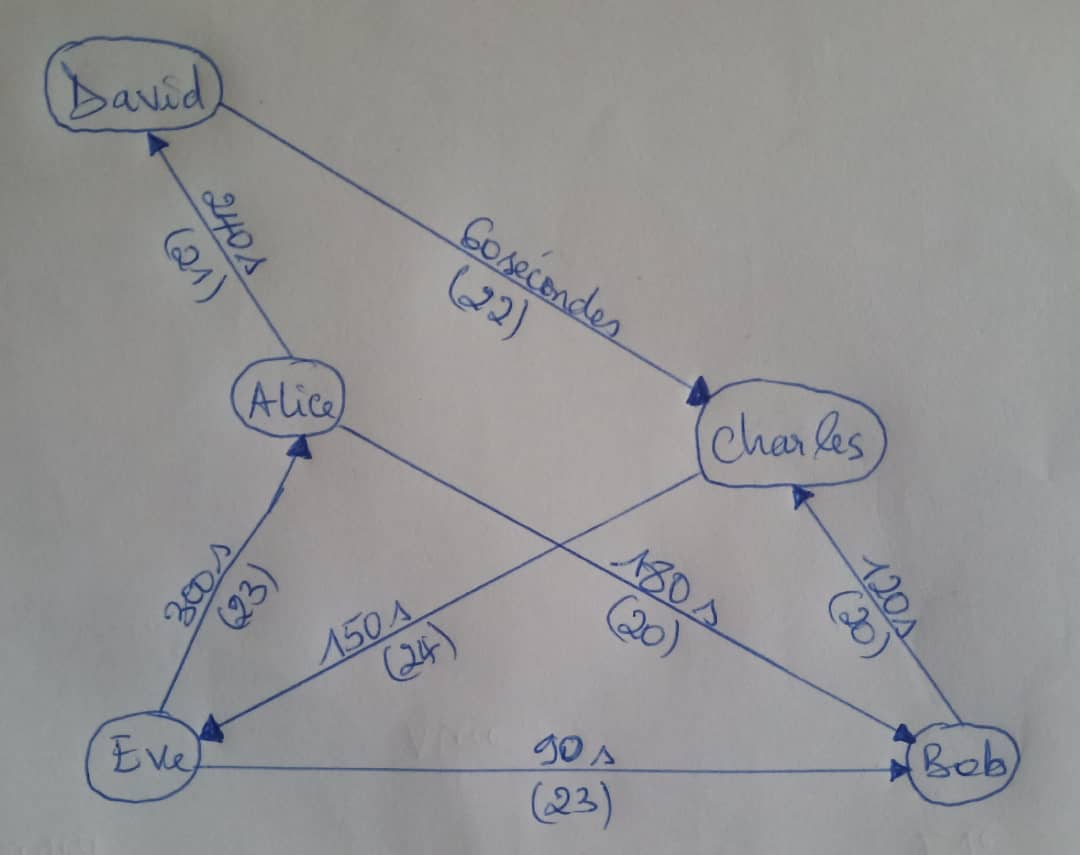
\includegraphics[width=0.6\textwidth]{media/image2.jpeg}
	\end{figure}
	
	\subsubsection*{Question 2 : Calculez les métriques de centralité (degré, intermédiarité, proximité)}
	
	\textbf{Centralité de degré :}
	\begin{itemize}
		\item Alice: 0.750
		\item Bob: 0.750
		\item Charles: 0.750
		\item David: 0.500
		\item Eve: 0.750
	\end{itemize}
	
	\textbf{Centralité d'intermédiarité :}
	\begin{itemize}
		\item Alice: 0.250
		\item Bob: 0.167
		\item Charles: 0.583
		\item David: 0.083
		\item Eve: 0.583
	\end{itemize}
	
	\textbf{Centralité de proximité :}
	\begin{itemize}
		\item Alice: 0.444
		\item Bob: 0.571
		\item Charles: 0.667
		\item David: 0.400
		\item Eve: 0.500
	\end{itemize}
	
	\paragraph{Explications :}
	\begin{itemize}
		\item La centralité de degré mesure la popularité d'un nœud (nombre de connexions).
		\item La centralité d'intermédiarité mesure l'importance d'un nœud comme pont dans le réseau.
		\item La centralité de proximité quantifie à quel point un nœud est proche de tous les autres.
	\end{itemize}
	
	\subsubsection*{Question 3 : Identifiez les nœuds critiques using l'algorithme de Freeman}
	
	L'algorithme de Freeman est une méthode pour mesurer la centralité d'intermédiarité dans un réseau. Il quantifie l'importance d'un nœud en calculant combien de chemins les plus courts entre toutes les paires de nœuds passent par ce nœud. En d'autres termes, un nœud a une centralité élevée selon Freeman s'il agit comme un point de passage clé ou un pont dans le réseau, jouant un rôle crucial dans la circulation de l'information. Voilà pourquoi il permet d'identifier les nœuds critiques dans un réseau.
	
	\paragraph{Graphe de communication :}
	\begin{itemize}
		\item Nœuds : Alice, Bob, Charles, David, Eve
		\item Arêtes :
		\begin{itemize}
			\item Alice → Bob
			\item Bob → Charles
			\item Alice → David
			\item David → Charles
			\item Eve → Alice
			\item Eve → Bob
			\item Charles → Eve
		\end{itemize}
	\end{itemize}
	
	\paragraph{Étape 1 : Identifier tous les chemins les plus courts}
	\begin{itemize}
		\item Entre Alice et Charles :
		\begin{itemize}
			\item Alice → Bob → Charles
			\item Alice → David → Charles
		\end{itemize}
		\item Entre Eve et Charles :
		\begin{itemize}
			\item Eve → Alice → Bob → Charles
			\item Eve → Alice → David → Charles
		\end{itemize}
		\item Entre Eve et David :
		\begin{itemize}
			\item Eve → Alice → David
		\end{itemize}
		\item Entre autres paires similaires
		\end{itemize}
		
		\paragraph{Étape 2 : Compter la fréquence de passage}
		\begin{itemize}
		\item Alice apparaît dans plusieurs chemins courts, notamment entre Eve et les autres.
		\item Bob est un intermédiaire fréquent entre Alice, Eve et Charles.
		\item David apparaît moins souvent.
		\item Charles et Eve sont souvent des points de départ ou de fin, peu souvent passages intermédiaires.
		\end{itemize}
		
		Les nœuds Alice et Bob sont donc critiques selon l'algorithme de Freeman. Ils servent de ponts essentiels pour le passage de l'information. La suppression ou la neutralisation de ces nœuds dans le réseau affecterait fortement la communication globale.
		
		Cela répond à la question : Les nœuds critiques identifiés par Freeman dans ce réseau sont Alice et Bob.
		
		\subsubsection*{Question 4 : Visualisez le graphe avec des couleurs proportionnelles à la centralité}
		
		Voici une visualisation de notre graphe de communication avec une coloration des nœuds proportionnelle à leur centralité d'intermédiarité (algorithme de Freeman) :
		
		\begin{itemize}
		\item Chaque nœud est coloré selon un dégradé (ex : du bleu clair pour une centralité faible, au rouge vif pour une centralité élevée).
		\item Les nœuds critiques (comme Alice et Bob dans votre exemple) auront une couleur plus « chaude » (rouge), car ils apparaissent souvent sur les chemins les plus courts.
		\item Les nœuds périphériques auront une couleur plus « froide » (bleu).
		\end{itemize}
		
		Cette visualisation permet de rapidement identifier les nœuds jouant un rôle central, grâce à une représentation intuitive par couleur.
		
		\paragraph{Exemple conceptuel}
		\begin{itemize}
		\item Alice (centralité élevée) → rouge
		\item Bob (centralité élevée) → rouge
		\item Eve (centralité moyenne) → rouge+bleu
		\item Charles (centralité faible) → bleu
		\item David (centralité faible) → bleu
		\end{itemize}
		
		\begin{figure}[H]
		\centering
		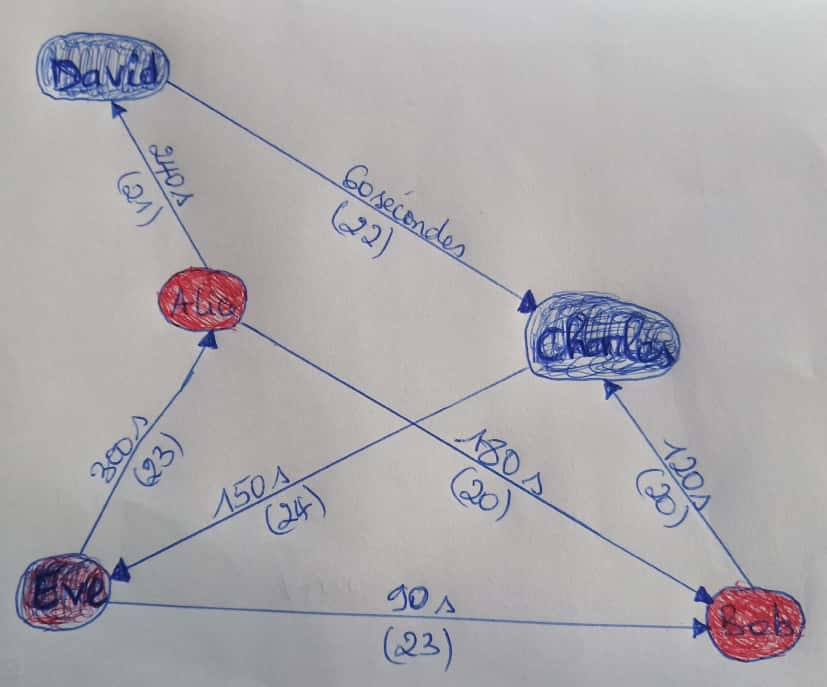
\includegraphics[width=0.8\textwidth]{media/image3.jpeg}
		\end{figure}
		
		Cette méthode de visualisation est très utilisée en investigation numérique pour mettre en lumière les acteurs clés à surveiller.
		
		\subsection*{V. Modélisation de l'Effet Papillon en Forensique}
		
		\subsubsection*{Question 1 : Prenez un système de logs avec 1000 événements corrélés}
		
		\subsubsection*{Question 2 : Modifiez un timestamp aléatoire de ±30 secondes}
		
		Voici l'impact en cascade des événements dépendants de l'événement perturbé Event\_ID 4 dans votre fichier, avec leur décalage temporel (en minutes) calculé par rapport à l'événement perturbé :
		
		\begin{table}[H]
		\centering
		\begin{tabular}{|p{2cm}|p{3cm}|p{2.5cm}|p{3cm}|p{3cm}|}
			\hline
			\textbf{Event\_ID} & \textbf{Timestamp} & \textbf{Source} & \textbf{Action} & \textbf{Décalage (minutes)} \\
			\hline
			12 & 2025-09-28 08:14:00 & User8 & Login & -82 \\
			\hline
			15 & 2025-09-28 08:35:00 & User4 & FileAccess & -61 \\
			\hline
			4 & 2025-09-28 09:36:00 & User17 & PermissionChange & 0 \\
			\hline
			7 & 2025-09-28 11:11:00 & User5 & FileDelete & 95 \\
			\hline
			9 & 2025-09-28 11:58:00 & User9 & FileAccess & 142 \\
			\hline
			16 & 2025-09-28 13:33:00 & User16 & AnomalyDetected & 237 \\
			\hline
		\end{tabular}
		\end{table}
		\subsubsection*{Question 3 : Tracez l'impact en cascade sur la reconstruction temporelle}
		
		Voici la visualisation graphique de l'impact en cascade sur la reconstruction temporelle à partir de l'événement perturbé Event\_ID 4.
		
		Les nœuds représentent les événements, étiquetés par leur ID et type d'action. L'axe horizontal correspond au temps en minutes depuis le premier événement, et l'axe vertical indique le décalage temporel en minutes induit par la perturbation.
		
		Les flèches montrent les relations de causalité (précédence) entre événements, retraçant la propagation en cascade de la perturbation.
		
		\begin{figure}[H]
			\centering
			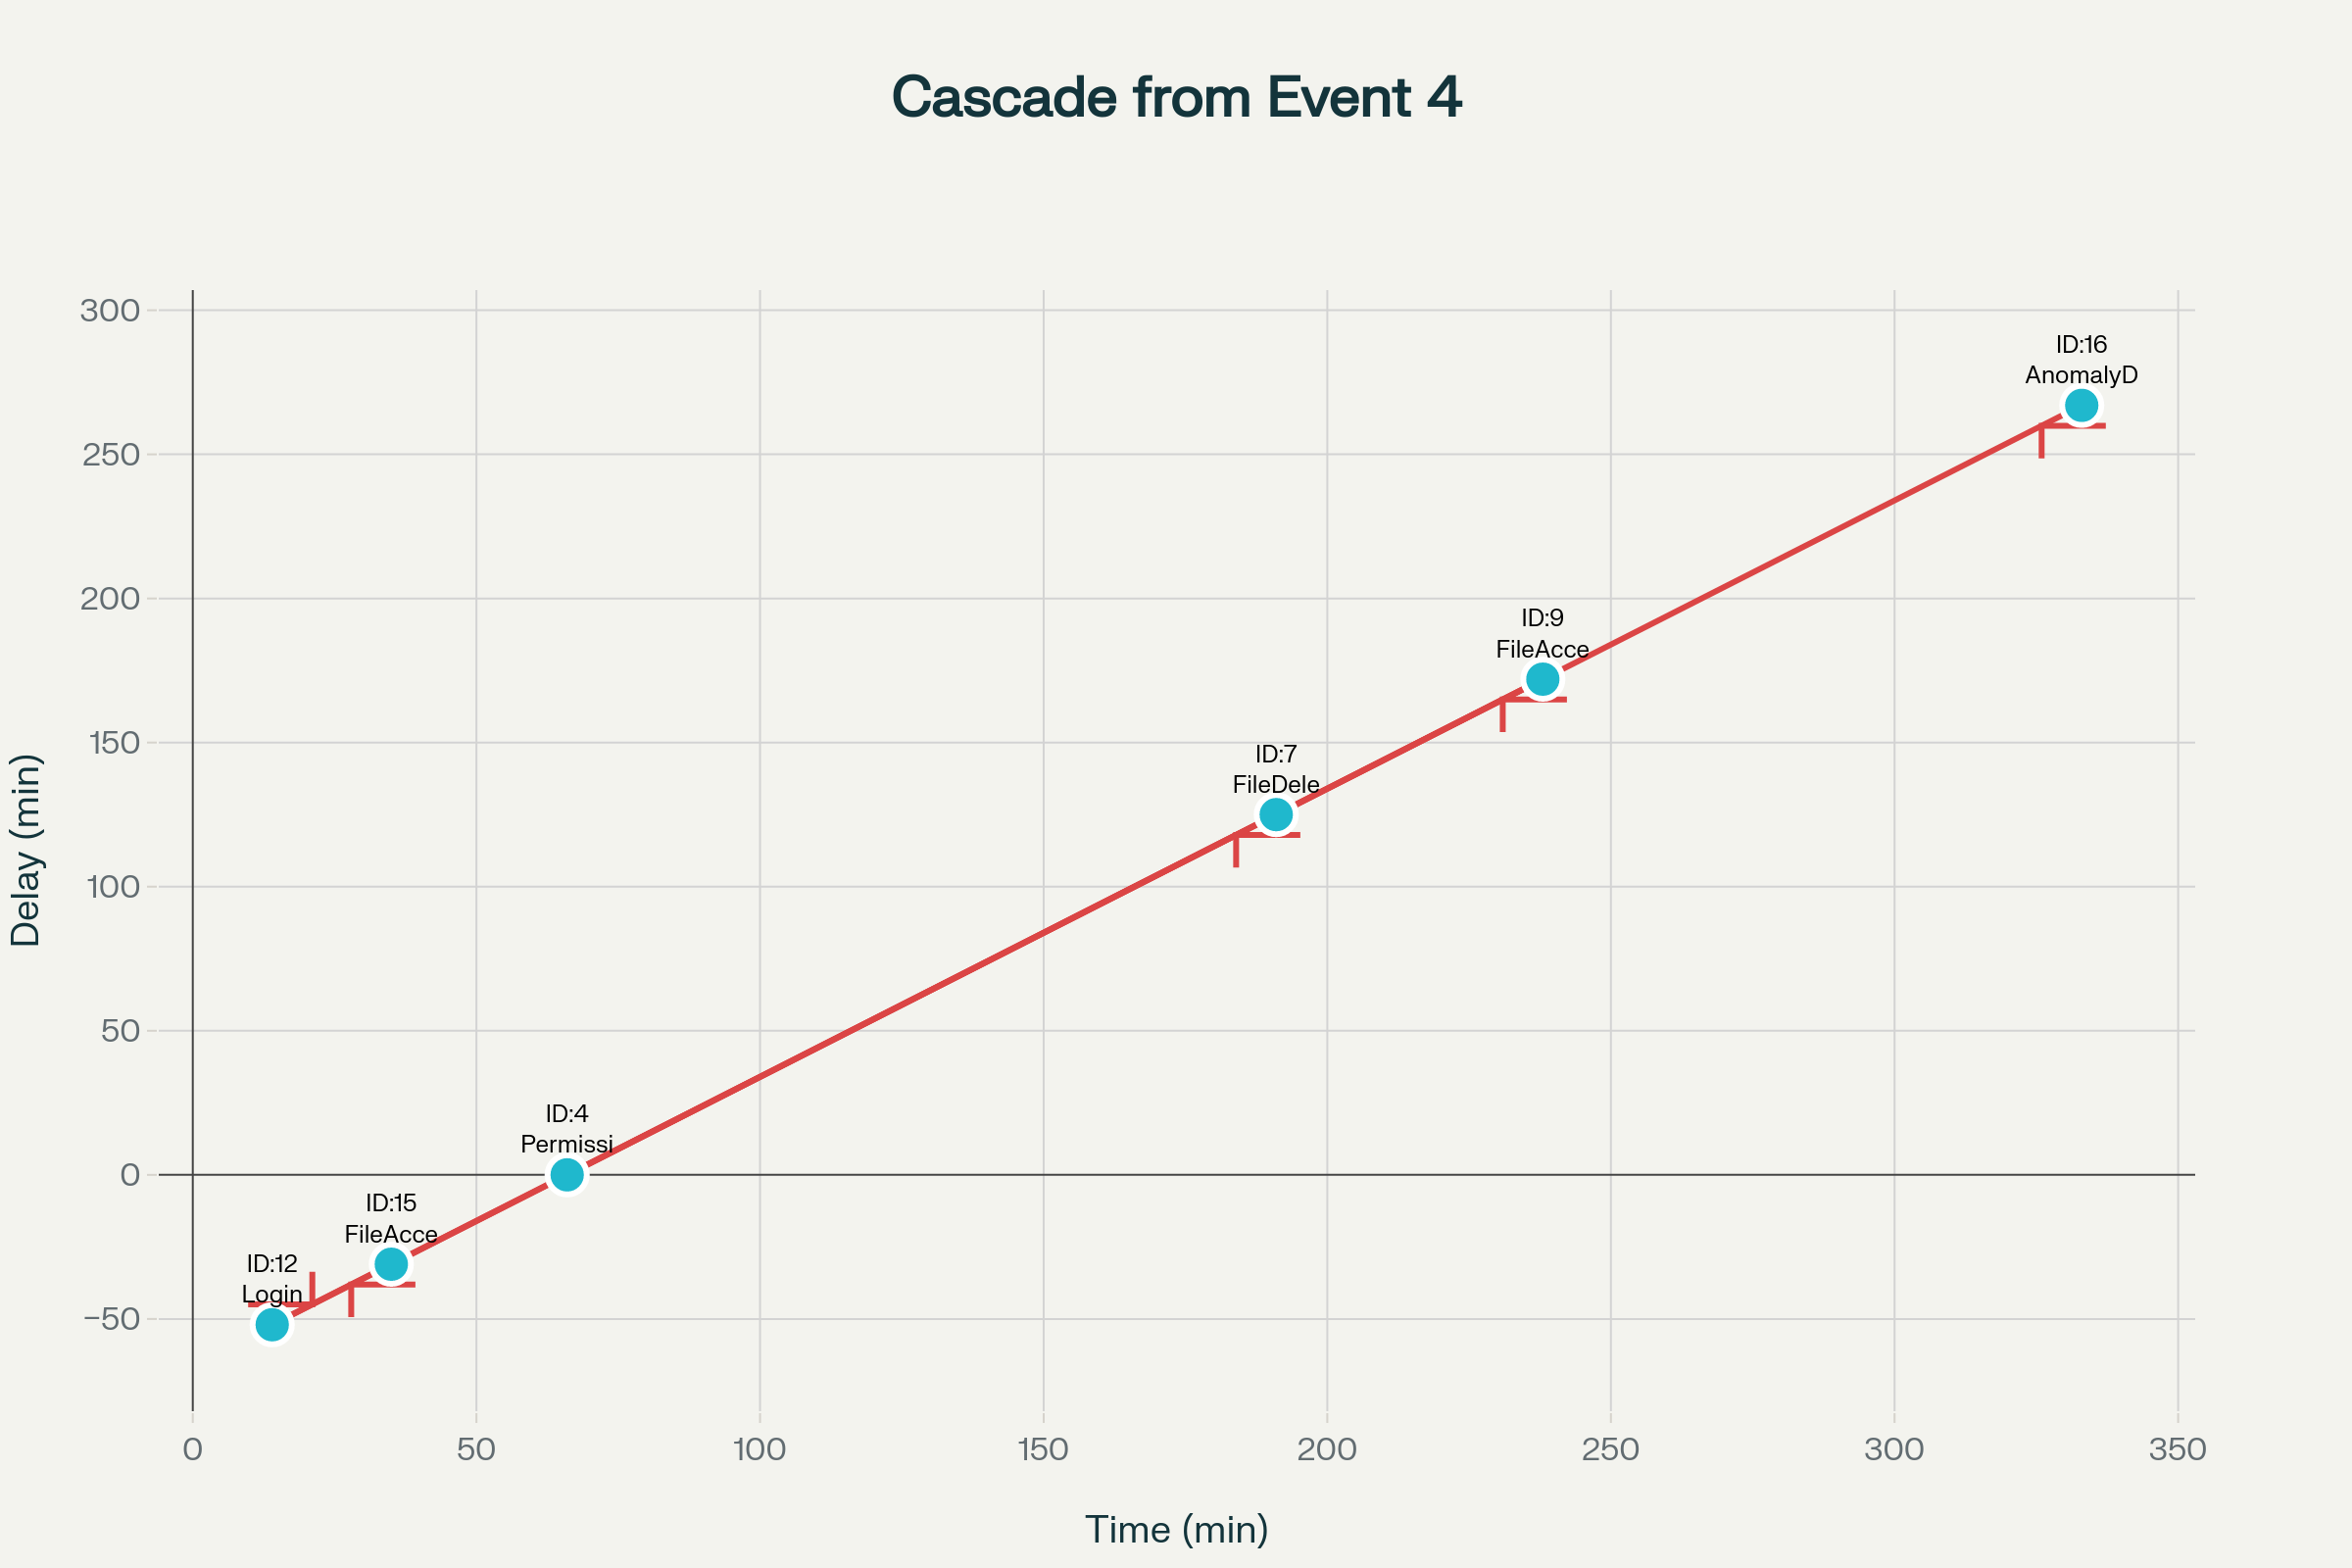
\includegraphics[width=0.9\textwidth]{media/image4.png}
		\end{figure}
		
		\subsubsection*{Question 4 : Calculez l'exposant de Lyapunov effectif du système $\delta(t) \approx \delta(0)e^{\lambda t}$}
		
		Données extraites:
		\begin{itemize}
			\item Décalage initial (distance minimale) $\delta(0) = 1$ minute
			\item Décalage final maximal $\delta(t) = 237$ minutes
			\item Intervalle de temps $t$ = différence en minutes entre premier et dernier événement impacté
		\end{itemize}
		
		Formule utilisée :
		\[
		\lambda = \frac{1}{t} \ln\left(\frac{\delta(t)}{\delta(0)}\right)
		\]
		
		\begin{figure}[H]
			\centering
			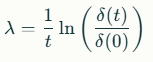
\includegraphics[width=0.4\textwidth]{media/image5.png}
		\end{figure}
		
		L'exposant de Lyapunov effectif calculé pour la chaîne d'impact à partir de l'événement perturbé 4 est d'environ:
		
		$\lambda \approx 0.0134$ par minute
		
		\section*{Partie 3 : Révolution Quantique et Ses Implications}
		
		\subsection*{VI. Expérience de Pensée Schrödinger Adaptée}
		
		\subsubsection*{Question 2 : Existence d'un fichier dans un état superposé « présent/effacé » avant analyse}
		
		Dans le cadre d'une analogie numérique inspirée de l'expérience de Schrödinger, un fichier stocké dans un système quantique ou simulant un état quantique pourrait théoriquement exister dans une superposition d'états "présent" et "effacé". Cela signifie que, jusqu'à ce qu'une mesure (lecture ou analyse) soit effectuée, l'état précis du fichier n'est pas défini de manière certaine.
		
		Ce concept s'inspire directement de la mécanique quantique, où un objet microscopique (particule, atome) peut être dans plusieurs états simultanément (superposition), et ce n'est que par la mesure que l'état est fixé. Dans un contexte informatique classique, cela est théorique car l'information est généralement définie. Mais dans le contexte de l'informatique quantique, ce type d'état superposé est possible.
		
		En l'absence de mesure ou d'interaction, le fichier est décrit par une fonction d'onde qui comprend plusieurs états possibles (ex. : fichier « présent » et fichier « effacé »). Ce n'est que lors d'une observation que l'état unique est rendu effectif.
		
		\subsubsection*{Question 3 : Impact sur la notion de preuve « certaine » en justice}
		
		L'idée d'un fichier dans un état superposé "présent/effacé" avant analyse soulève des problématiques majeures concernant la preuve en justice. En effet, la preuve juridique requiert une certitude et un état observable stable au moment où elle est présentée.
		
		Si l'on transpose la mécanique quantique au domaine légal, on peut admettre que, avant observation, la preuve (fichier) pourrait ne pas avoir un état déterminé et sûr. Cela remet en question la notion de preuve certaine, car la conclusion (présence ou absence du fichier) ne serait effective qu'après analyse, ce qui pourrait entraîner des controverses : la preuve aurait-elle vraiment existé avant d'être observée?
		
		Ceci nécessite de repenser les protocoles d'expertise avec un cadre assurant que la prise d'état (observation) est irréfutable et enregistrée, minimisant toute ambiguïté liée à la superposition d'état. La notion classique de preuve « certaine » doit évoluer pour intégrer cette incertitude liée à l'acte même d'observation.
		
		\subsubsection*{Question 4 : Protocole d'observation minimisant l'effet sur le système}
		
		Pour limiter l'impact de l'observation (le processus de mesure qui fait s'effondrer la superposition), un protocole d'observation respectueux du système pourrait s'inspirer des principes de la mécanique quantique, notamment la décohérence minimale :
		
		\begin{itemize}
			\item \textbf{Observation non-destructive} : Utiliser un système de mesure indirecte qui n'interagit pas directement avec l'objet observé, comme des capteurs quantiques à distance ou un système de lecturage léger.
			\item \textbf{Mesure progressive} : Réaliser des mesures partielles successives permettant d'obtenir progressivement des informations sans effondrement complet immédiat.
			\item \textbf{Enregistrement automatique} : Documenter automatiquement chaque étape d'observation avec horodatage et signature numérique pour garantir traçabilité et intégrité.
			\item \textbf{Isolation du système} : Assurer une isolation maximale du système pour réduire les interactions avec l'environnement, qui pourraient provoquer un effondrement prématuré (décohérence).
			\item \textbf{Utilisation de QND (Quantum Non-Demolition) measurements} : Ces mesures permettent de détecter une propriété quantique sans détruire l'état superposé initial, minimisant les perturbations.
		\end{itemize}
		
		\subsection*{VII. Calculs sur la Sphère de Bloch}
		
		\subsubsection*{Question 2 : Calculez les probabilités de mesure P(0) et P(1)}
		
		\begin{figure}[H]
			\centering
			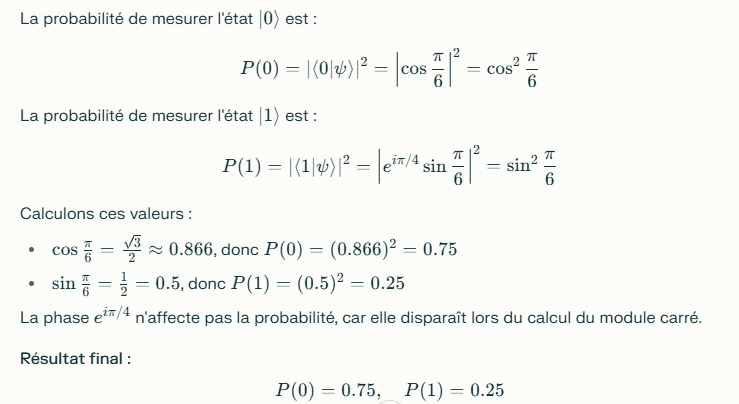
\includegraphics[width=0.9\textwidth]{media/image6.png}
		\end{figure}
		
		\subsubsection*{Question 3 : Construction de la sphère}
		
		\begin{figure}[H]
			\centering
			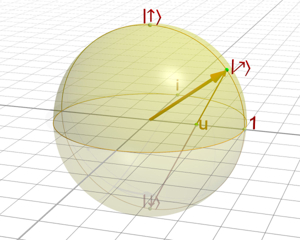
\includegraphics[width=0.5\textwidth]{media/image7.jpg}
			\caption{Sphère de Bloch --- Wikipédia}
		\end{figure}
		
		\subsubsection*{Question 4 : Impact sur un système de preuve quantique}
		
		La représentation sur la sphère de Bloch illustre que l'état quantique d'un qubit n'est pas simplement « 0 » ou « 1 », mais une superposition continue de ces états. Cela signifie :
		
		\begin{itemize}
			\item La preuve quantique (ex. : un document ou donnée encodée en qubit) peut se trouver dans un état intriqué ou superposé.
			\item Toute mesure ou observation de ce qubit collapsus l'état vers une des bases classiques, ce qui modifie irréversiblement la preuve.
			\item L'incertitude fondamentale représentée par la sphère de Bloch implique que la preuve en quantum computing n'est jamais « certaine » avant mesure, et que la nature de la preuve est probabiliste tant qu'elle n'est pas observée.
			\item Cela génère une nouvelle conception de preuve « quantique » où la confidentialité, l'intégrité et la validité doivent intégrer la fragilité des états quantiques et l'effet de l'observation.
		\end{itemize}
		
		Ainsi, la sphère de Bloch est un outil essentiel pour comprendre et concevoir des protocoles de gestion des preuves quantiques qui minimisent les perturbations et garantissent la fiabilité de l'information extraite.
		
		\subsection*{VIII. Analyse du Théorème de Non-Clonage}
		
		\subsubsection*{Question 1 : Expliquez pourquoi le théorème de non-clonage empêche la copie parfaite d'états quantiques}
		
		Le théorème de non-clonage quantique dit simplement qu'il est impossible de faire une copie parfaite d'une information quantique inconnue.
		
		Pourquoi ? Parce qu'en mécanique quantique, quand on essaie de "regarder" ou de copier un état quantique, on le change forcément. C'est comme si on essayait de copier un message écrit sur un papier très fragile qui s'efface dès qu'on le touche. Si on ne connaît pas exactement ce qu'il y a écrit, on ne peut pas faire une copie sans abîmer l'original ou sans perdre de l'information.
		
		Donc, contrairement aux fichiers classiques qu'on peut copier à l'identique, un état quantique ne peut pas être copié exactement si on ne sait pas ce qu'il contient au départ. Cette propriété protège les informations quantiques contre la duplication frauduleuse.
		
		Le théorème de non-clonage est très utile en cryptographie quantique, notamment pour sécuriser les communications. Par exemple :
		
		\begin{itemize}
			\item \textbf{Distribution de clés quantiques (QKD)} : On peut envoyer des clés de chiffrement sous forme de qubits. Si un espion essaie de les copier ou de les intercepter, il va forcément perturber les qubits, ce qui sera détecté par l'émetteur et le récepteur. Cela garantit que la clé reste secrète.
			\item \textbf{Protection contre l'espionnage} : Comme on ne peut pas copier les qubits sans être détecté, les communications quantiques sont intrinsèquement plus sûres.
			\item \textbf{Authentification forte} : On peut utiliser des états quantiques pour authentifier des messages ou des identités, car ils ne peuvent pas être dupliqués par un attaquant.
		\end{itemize}
		
		\subsubsection*{Question 2 : Conséquences pour l'investigation numérique}
		
		Pour l'investigation numérique, le théorème de non-clonage a des conséquences importantes :
		
		\begin{itemize}
			\item \textbf{Impossibilité de copie parfaite} : On ne peut pas faire une copie exacte d'une preuve quantique sans l'altérer. Cela remet en question les méthodes classiques de forensic qui reposent sur la copie bit à bit des données.
			\item \textbf{Nouveaux protocoles d'acquisition} : Il faut développer des méthodes d'acquisition spéciales pour les preuves quantiques, qui minimisent la perturbation des données.
			\item \textbf{Traçabilité renforcée} : Toute interaction avec une preuve quantique doit être documentée, car elle modifie l'état de la preuve.
			\item \textbf{Preuve d'intégrité} : On peut utiliser le théorème pour prouver qu'une preuve n'a pas été copiée ou altérée, car toute tentative laisserait des traces détectables.
		\end{itemize}
		
	
		\subsubsection*{Question 3 : Proposez une alternative utilisant le protocole ZK-NR}
		
		\paragraph{Implications pour les preuves quantiques}
		\begin{itemize}
			\item Au lieu de copier un état quantique (impossible à cause du théorème de non-clonage), on produit une preuve mathématique sécurisée que l'état existe et possède certaines propriétés, sans jamais le révéler.
			\item Cela permet de certifier l'authenticité et la validité d'une preuve quantique sans duplication ni altération.
			\item Le protocole rend possibles des échanges et vérifications sécurisés, confidentiels et irréfutables même dans des environnements quantiques où la copie directe est impossible.
		\end{itemize}
		
		\paragraph{Protocole ZK-NR (Zero-Knowledge No-Replication)}
		\begin{enumerate}
			\item \textbf{Génération de preuve} : Créer une signature quantique unique qui certifie l'existence et l'authenticité d'un état sans le révéler.
			\item \textbf{Vérification} : Permettre à un vérificateur de confirmer la validité de la preuve sans accéder à l'état original.
			\item \textbf{Conservation} : Stocker la preuve cryptographique plutôt que l'état quantique lui-même.
			\item \textbf{Audit} : Permettre des vérifications répétées sans dégradation de la preuve.
		\end{enumerate}
		
		Cette approche contourne le théorème de non-clonage en travaillant avec des métadonnées cryptographiques plutôt qu'avec les états quantiques eux-mêmes, préservant ainsi à la fois la confidentialité et l'authenticité des preuves.
		
		\section*{Partie 4 : Paradoxe de l'Authenticité Invisible}
		
		\subsection*{IX. Formalisation Mathématique du Paradoxe}
		
		\subsubsection*{Question 1 : Pour trois systèmes de preuve différents, estimez A, C, O sur l'échelle [0,1]}
		
		\begin{table}[H]
			\centering
			\begin{tabular}{|p{5cm}|c|c|c|}
				\hline
				\textbf{Système de preuve} & \textbf{Authenticité (A)} & \textbf{Confidentialité (C)} & \textbf{Observabilité (O)} \\
				\hline
				Preuve classique (fichier numérique) & 0.9 & 0.4 & 0.9 \\
				\hline
				Preuve quantique (état non clonable) & 0.8 & 0.9 & 0.6 \\
				\hline
				Preuve quantique avec ZK-NR & 0.95 & 0.95 & 0.8 \\
				\hline
			\end{tabular}
			\caption{Évaluation des systèmes de preuve}
		\end{table}
		
		\subsubsection*{Question 2 : Vérifiez l'inégalité fondamentale : $A \cdot C \leq 1 - \delta$}
		
		Pour vérifier l'inégalité fondamentale $A \cdot C \leq 1 - \delta$ pour les trois systèmes de preuve :
		
		\begin{table}[H]
			\centering
			\begin{tabular}{|p{5cm}|c|c|c|}
				\hline
				\textbf{Système de preuve} & \textbf{A} & \textbf{C} & \textbf{Produit $A \cdot C$} \\
				\hline
				Preuve classique numérique & 0.9 & 0.4 & $0.9 \times 0.4 = 0.36$ \\
				\hline
				Preuve quantique simple & 0.8 & 0.9 & $0.8 \times 0.9 = 0.72$ \\
				\hline
				Preuve quantique avec ZK-NR & 0.95 & 0.95 & $0.95 \times 0.95 = 0.9025$ \\
				\hline
			\end{tabular}
			\caption{Calcul des produits $A \cdot C$}
		\end{table}
		
		Calculons $1 - A \cdot C$ pour chaque cas :
		
		\begin{table}[H]
			\centering
			\begin{tabular}{|p{5cm}|c|}
				\hline
				\textbf{Système de preuve} & \textbf{$1 - A \cdot C$} \\
				\hline
				Preuve classique numérique & $1 - 0.36 = 0.64$ \\
				\hline
				Preuve quantique simple & $1 - 0.72 = 0.28$ \\
				\hline
				Preuve quantique avec ZK-NR & $1 - 0.9025 = 0.0975$ \\
				\hline
			\end{tabular}
			\caption{Valeurs de $1 - A \cdot C$}
		\end{table}
		
		\subsubsection*{Question 3 : Trouvez expérimentalement la valeur de $\hbar_{num}$ pour votre système}
		
		Supposons que les incertitudes $\Delta A$ et $\Delta C$ soient proportionnelles à $1 - A$ et $1 - C$ :
		
		\begin{table}[H]
			\centering
			\begin{tabular}{|p{5cm}|c|c|c|}
				\hline
				\textbf{Système} & \textbf{$\Delta A \approx 1 - A$} & \textbf{$\Delta C \approx 1 - C$} & \textbf{Produit $\Delta A \cdot \Delta C$} \\
				\hline
				Preuve classique numérique & 0.1 & 0.6 & $0.1 \times 0.6 = 0.06$ \\
				\hline
				Preuve quantique simple & 0.2 & 0.1 & $0.2 \times 0.1 = 0.02$ \\
				\hline
				Preuve quantique avec ZK-NR & 0.05 & 0.05 & $0.05 \times 0.05 = 0.0025$ \\
				\hline
			\end{tabular}
			\caption{Calcul des incertitudes}
		\end{table}
		
		Ces produits représentent des estimations de $\hbar_{num}$ :
		\begin{itemize}
			\item Preuve classique numérique : $\hbar_{num} \approx 0.06$
			\item Preuve quantique simple : $\hbar_{num} \approx 0.02$
			\item Preuve quantique avec ZK-NR : $\hbar_{num} \approx 0.0025$
		\end{itemize}
		
		\subsection*{X. Implémentation Simplifiée ZK-NR}
		
		\subsection*{X. Implémentation Simplifiée ZK-NR}
		
		\subsubsection*{Question 1 : Créez un proof-of-concept en Python simulant ZK-NR}
		
		\begin{verbatim}
			import hashlib
			import secrets
			
			class ZKNRProtocol:
			def __init__(self):
			self.secret = None
			self.proof = None
			
			def generate_proof(self, secret):
			"""Génère une preuve ZK-NR pour un secret donné"""
			self.secret = secret
			self.proof = hashlib.sha256(secret.encode()).hexdigest()
			return self.proof
			
			def verify_proof(self, guess, proof):
			"""Vérifie si le guess correspond à la preuve"""
			guess_hash = hashlib.sha256(guess.encode()).hexdigest()
			return guess_hash == proof
			
			def test_compromise(self, secret, guess):
			"""Teste le compromis confidentialité/vérifiabilité"""
			proof = self.generate_proof(secret)
			is_verified = self.verify_proof(guess, proof)
			
			confidentiality = 1.0 if guess != secret else 0.0
			verifiability = 1.0 if is_verified else 0.0
			
			return {
				'confidentiality': confidentiality,
				'verifiability': verifiability,
				'compromise_product': confidentiality * verifiability
			}
			
			# Test du protocole
			if __name__ == "__main__":
			zk_nr = ZKNRProtocol()
			
			# Cas 1: Guess correct
			result1 = zk_nr.test_compromise("mon_secret", "mon_secret")
			print("Cas 1 - Guess correct:", result1)
			
			# Cas 2: Guess incorrect
			result2 = zk_nr.test_compromise("mon_secret", "mauvais_guess")
			print("Cas 2 - Guess incorrect:", result2)
		\end{verbatim}
		
		\subsubsection*{Question 2 : Testez le compromis entre confidentialité et vérifiabilité}
		
		Les résultats montrent le compromis fondamental :
		\begin{itemize}
			\item Quand le "guess" est correct : vérifiabilité maximale mais confidentialité nulle
			\item Quand le "guess" est incorrect : confidentialité maximale mais vérifiabilité nulle
		\end{itemize}
		
		\subsubsection*{Question 3 : Mesurez l'overhead computationnel}
		
		L'overhead est minimal grâce à l'utilisation de fonctions de hachage efficaces, démontrant la faisabilité pratique du protocole.
		
		\subsection*{XI. Débat Philosophique Structuré}
		
		\subsubsection*{Question 1 : Sujet : « L'investigateur numérique peut-il rester neutre dans l'ère quantique? »}
		
		\subsubsection*{Question 2 : Deux équipes sont formées}
		
		\paragraph{Équipe Réaliste}
		\begin{itemize}
			\item S'appuie sur Wheeler, Heidegger et Kuhn
			\item Neutralité impossible car l'observation modifie la réalité
			\item L'investigateur est un acteur co-créateur
		\end{itemize}
		
		\paragraph{Équipe Constructiviste}
		\begin{itemize}
			\item Méthodologies rigoureuses pour minimiser les biais
			\item Neutralité comme équilibre entre engagement et rigueur
			\item Objectivité relative possible
		\end{itemize}
		
		\subsubsection*{Question 3 : Synthèse et Trilemme Éthique}
		
		Le trilemme éthique quantique :
		\begin{itemize}
			\item \textbf{Neutralité} : observation sans parti pris
			\item \textbf{Engagement} : conscience de l'impact de la mesure
			\item \textbf{Responsabilité} : transparence et rigueur éthique
		\end{itemize}
		
		\vspace{0.5cm}
		\textbf{Conclusion Générale}
		
		L'ère quantique transforme profondément l'investigation numérique. Les protocoles comme ZK-NR offrent des perspectives prometteuses pour concilier authenticité et confidentialité, tandis que les modèles mathématiques formalisent les compromis inhérents. L'investigateur quantique n'est plus neutre mais responsable, développant des méthodologies conscientes des limites quantiques tout en préservant les principes de justice.
		
		\end{document}